
\section{INTRODUCTION} 
During the latest stage of structure formation, the universe gave birth to
non-linear, hierarchical structures known as galaxy clusters. 
These clusters, made up of dark matter, galaxies and hot gas,
are constantly accreting mass, merging and evolving with their
environments. Bright galaxies that belong to a galaxy cluster or group, in 
particular, highlight the overdensities of the underlying dark matter (DM) 
distribution. 

% Peaks, summary statistics 
% Modeling galaxy clusters - distributions, peaks, centroids 

In these dense regions of the clusters, the rates of particle
interactions can be enhanced, including the long-suspected self-interaction of DM
particles (hereafter, SIDM).  
Many papers have used the offsets between the summary statistics of the DM
density and the galaxy density to give constraints on 
the self-interaction cross
section, i.e. $\sigma_{\rm SIDM}$, of dark matter. 
A lot of observational studies focus on using merging galaxy clusters
as they assume the high collisional velocity should further increase the chance
of detecting the effects of SIDM.
By assuming galaxies being relatively collisionless $\sigma_{\rm gal} \approx 0$, 
any offset of the DM population from the galaxy provides $\sigma_{\rm SIDM}$ 
relative to $\sigma_{\rm gal} \approx 0 \centi\meter^2$. 
These observational studies include \cite{Markevitch2004} and \cite{Bradac2006b}  
reporting an offset of 25 kpc for the Bullet Cluster;  
\cite{Dawson2013} reporting an offset of 129 kpc and 47 kpc for the southern
and the northern subcluster respectively;
\cite{Jee2015} reporting an offset of 190 kpc for MACSJ1752, and others that we
list in detail in table [TODO].
However, other studies using 129 X-ray selected relaxed galaxy clusters, 
such as \cite{George2012a} also report offsets of the same order of magnitude,
between $50 - 150$ kpc. 

On the other hand, there are many staged simulations of mergers of galaxy
clusters that focused on detecting the signal from
SIDM. These staged simulation usually have parametric prescriptions of the 
spatial distribution of galaxies  
(\citealt{Randall2008d}, \citealt{Kahlhoefer14}, \citealt{Robertson2016}), 
such as an NFW profile, 
and do not have realistic galaxy features, nor dynamical
frictions. 
They try to show the magnitude of offsets solely due to SIDM \citep{Kahlhoefer14} as 
by initializing the galaxy-DM offset to be zero at the beginning of their 
simulations. 
Furthermore, these staged simulations commonly use a much higher number of 
galaxy particles than the realistic observable number of galaxies. 
\cite{Randall2008d} found an offset of only 1.8 kpc in the staged merger
simulation with $\sigma_{\rm SIDM} = 0 \centi\meter^2 /$ g using $10^5$ 
galaxy particles 
When assumed with zero impact parameter for mergers, Kim and Peter et al.
(2016), using 5.7k or 57K galaxy tracer particles also show 
null galaxy-DM offset during most periods of their control staged simulation 
with $\sigma_{\rm
SIDM} = 0 \centi\meter^2 /$ g. While we provide a more in-depth comparison with
these staged simulation in the discussion, we argue 
these staged simulations do not probe  
how statistical and observational uncertainties realistically contribute to 
the galaxy-DM offsets. 
As such, any offsets 
from aforementioned staged simulations when they increased $\sigma_{\rm
SIDM}$, they can guarantee the offsets are maximally due to SIDM.
When these simulations set the $\sigma_{\rm SIDM}$ to observationally motivated 
levels of $< 3$ \centi\meter$^2$/g, 
different authors have consistently reported offset signals  
on par with uncertainties estimated from individual observations. 
These simulations have raised questions about how strongly the galaxy-DM offsets 
can constrain the effects of SIDM.
When \cite{Kahlhoefer14} simulated SIDM with both low-momentum-transfer 
self-interaction 
and rare self-interactions of DM with high momentum transfer, they found maximum 
offsets that are $< 30$ kpc for $\sigma_{\rm SIDM}$ as high as 1.6
\centi\meter$^2$ / \gram.
The reported offset from \cite{Randall2008d}
for $\sigma_{\rm SIDM} = 1.24 \centi\meter^2 / \gram$ is only 53.9 kpc. 
While [TODO] Kim and Peter et al. (2016) found a maximum offset $< 50$ kpc for 
$\sigma_{\rm SIDM} = 3 \centi\meter^2 / \gram$ ,
and \cite{Robertson2016} also found a maximum offset $\lesssim 50$ kpc  
 from a simulation suite of a Bullet Cluster analog 
 with $\sigma_{\rm SIDM} = 1~\centi\meter^2 /$ \gram.

An alternative explanation for the observed galaxy-DM offsets is due to 
statistical and observational uncertainties. Galaxies are very
sparse samples of the underlying DM overdensities, it is possible that the 
summary statistic of the sparse sample be different from those of the 
underlying distribution. It is not clear if there is any physical
cause of the galaxy-DM offset in a CDM universe, 
but any statistical noise leading to an offset can influence this method of 
the inference of $\sigma_{\rm SIDM}$. 
Since the Illustris simulation assumes no SIDM, this study is complementary to 
staged simulation for understanding what can contribute to the offsets.
% We therefore, perform mock observations of the galaxies clusters of the
% Illustris simulation to characterize the intrinsic scatter of the offsets.  
Simply put, we perform a hypothesis test with the galaxy-DM offsets in
the Illustris simulation directly corresponding to our null hypothesis
$\mathcal{H}_0$, with: 
\begin{equation}
\begin{cases}
	\text{the null hypothesis }\mathcal{H}_0: \text{Cold Dark Matter (CDM)} \\
	\text{the alternative hypothesis }\mathcal{H}_1: \text{Self-interacting Dark
	Matter (SIDM)} 
\end{cases}
\end{equation}

% This is the first study to compare the magnitude of SIDM offset signal with
% statistical noise, such as projection effects and unknown dynamical history. 
% These latent variables are confounding and can increase the variance of
% the population distribution of the galaxy-DM offsets.  

This exercise is further complicated by the fact that there is no theoretical
foundation showing which observable would be the most sensitive to each
possible type of SIDM. In fact, \cite{Kahlhoefer14} have argued that SIDM 
does not cause
significant offsets between the galaxy and DM peaks, and only cause an offset
between the corresponding centroids for a brief period of time after a merger. 
% To access if the offsets we observe is
% completely explained by the method for computing the offset, we investigate   
% the precision to which we can find the galaxy-DM offsets.  
Popular choice for computing the offsets involves first inferring the summary
statistic of the DM population and those of the galaxy population of a cluster
independently before taking a difference.
While there are well established procedures driven by lensing physics for 
inferring the DM spatial distribution, there is no standard procedure for
mapping the sparse member galaxy distribution. 
We quantify the bias and uncertainty associated with the one-point summary
statistic for summarizing member galaxy population. 
% 
% % What are the observational methods for summarizing dark matter distribution?
% % Weak and strong lensing are the most reliable methods for mapping the dark 
% % matter distribution in a galaxy cluster. 
% % Common to all the methods are the estimation of the density peaks. 
% % Uncertainties affect the conclusion for the computation the hypothesis test / parameter
% % estimation
% % Previous work on quantifying galaxy-DM offsets included  
% % What centroids they have used
% % 
% % Physical motivation for using the galaxy density peak 
% % Observation footprints 
% % 
% % Under the assumed Lambda Cold Dark Matter ($\Lambda$CDM) cosmology, it is unclear 
% % that how large the offset $\Delta \vec{s}$ should be. 
% % % Why use simulation data to study the populations? 
% % Other complications for studying galaxy clusters arise from observation
% % limitations. There is not a lot of information that can help constrain the  
% % line-of-sight distance of different components of a cluster. 
% 
% 
% % Goals of the paper
% % With the advent of large-scale optical sky surveys, 
% % the number of identified galaxy clusters is growing quickly. 
% % Existing catalogs such as the Abell catalog also contain
% % peaks inferred
% % from the different peak finding methods and the DM peaks. 
% % at least 4000 clusters with at least 30 members. 
% % The future Large Synoptic Sky Survey alone will identify over a hundred thousand galaxy
% % clusters (CITE) in optical wavelengths. 
% % It is important to verify the uncertainties associated with common
% % summary statistics for studying galaxy clusters. Considering the large quantity
% % of data, methods with manual tuning will not scale well. The manual biases may
% % also make it hard to obtain consistent statistics from the samples.

In this paper, we 
1) extract realistic observables from the Illustris simulation for
comparison with observations, 2) explore the pros and cons of the different statistic for 
summarizing {\it the member galaxy population} of a galaxy cluster, 3)	
give estimates for the offsets between the summary statistics of the galaxy  
population and the DM population under $\Lambda$CDM cosmology, which we call 
\begin{equation}
	\Delta \vec{s} \equiv \vec{s}_{\rm gal} - \vec{s}_{\rm DM}.
\end{equation}
where $\bf{s}_{gal}$ and $\bf{s}_{DM}$ are the two-dimensional (2D) spatial
locations of the summary statistic of the galaxy population, and the density
peak of DM respectively. This gives
an estimate of the baseline scatter of offsets without any SIDM. And finally we 
4) examine the properties of the clusters that give outliers in 
the offset distribution and 5) investigate the  
correlations between the physical properties of a cluster and the projected 
observables such as $\Delta s$. 
\begin{figure*}
	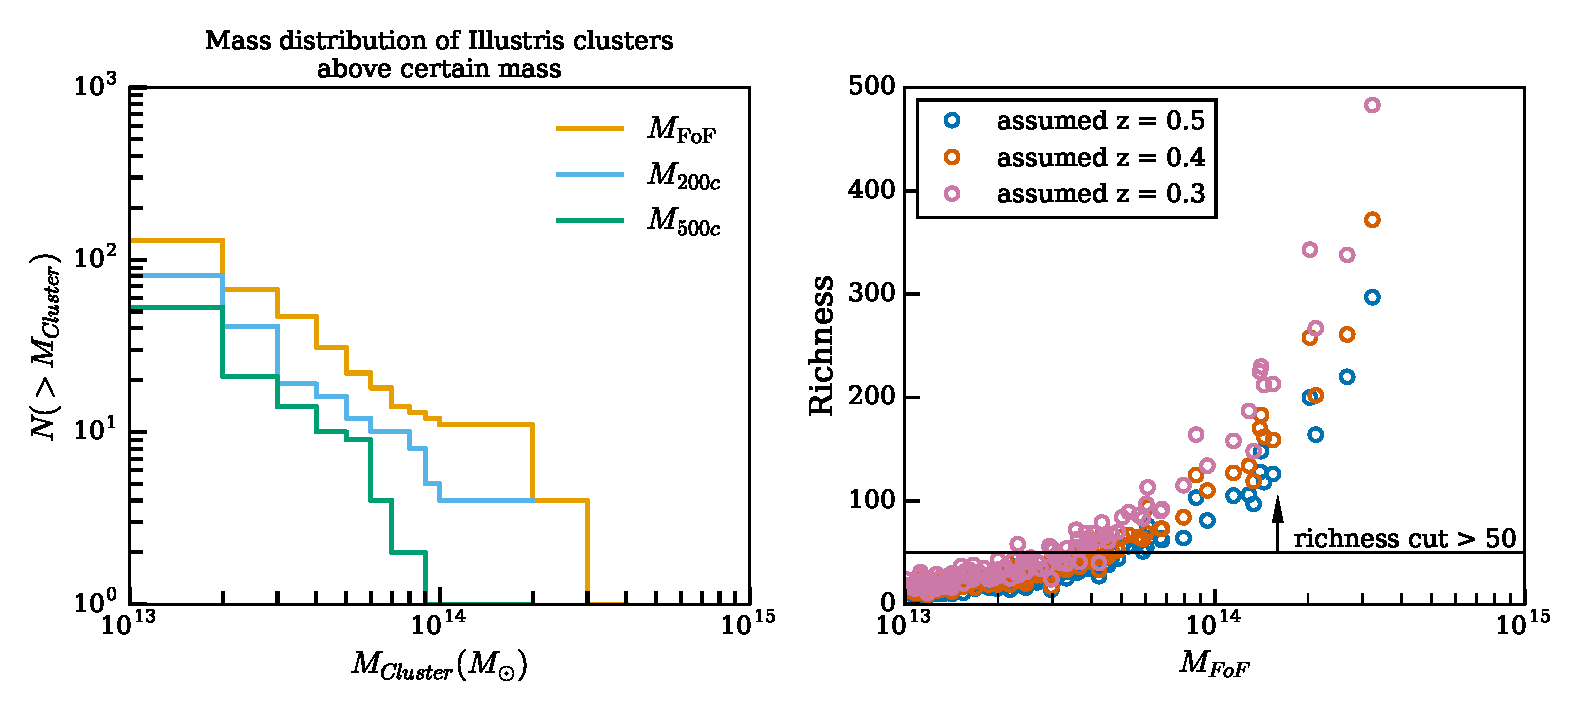
\includegraphics[width=\linewidth]{fig1_mass_richness.eps}
	\caption{ {\bf Left figure:} Mass distribution of the group / cluster sized 
		DM halos for different halo selection schemes. Mass estimates obtained by the
		FoF algorithm are labeled as  M$_{\text{FoF}}$.
		Masses centered on the most bound particle within a radius those the 
		average density is 200 or 500 times the critical density of the universe are 
		labeled as M$_{200c}$ and M$_{500c}$ respectively. 
		% Huge discrepancies between the $M_{500c}$ and $M_{\rm FoF}$ of the clusters 
		% indicate the presence of spatially
		% separated substructures for the clusters (See Fig. 
		% \ref{fig:select_peak_visualization}). 
		{\bf Right figure:} 
		Mass-richness relationship of galaxy clusters and groups with 
		$M_{\rm FoF} > 10^{13} M_{\odot}$ assuming different cosmological redshifts
		of the observed clusters. 
\label{fig:mass_richness}}
\end{figure*}

% Basic setup 
The organization of this paper is as follows:
In section \ref{sec:illustris_sim}, we will describe the physical properties of 
the data of the Illustris
simulation (\citealt{Vogelsberger2014}, \citealt{Genel2014a}), 
and the selection criteria that we have employed to ensure that the
quantities that we examine resemble observables but without noise and
systematics from observations. 
Then in section \ref{sec:methods}, 
we explain the methods for computing various 
one-point statistics of the spatial distribution of galaxies how we prepare our dark
matter spatial data to resemble convergence maps. We show the statistical performance
of the different summary statistics before we show the main results
in section \ref{sec:results}. In the discussion in section \ref{sec:discussion}, 
we list the implications of our
results and compare it to other simulations and observations. We also 
show how one may make use of the population offset statistical distribution
from the Illustris data to construct a test with 
a null hypothesis of $\sigma_{\rm SIDM} = 0$ and discuss the caveats. 

	Our analysis makes use of the same flat Lambda Cold Dark Matter ($\Lambda$CDM) cosmology
as the Illustris simulation. The relevant cosmological parameters are
$\Omega_\Lambda = 0.7274, \Omega_m = 0.2726$, and $H_0 = 70.4$
km~s$^{-1}$~Mpc$^{-1}$.

\section{THE ILLUSTRIS SIMULATION DATA} 
\label{sec:illustris_sim}
The Illustris simulation contains some of the most
realistic, simulated galaxies to date, making it especially suitable for 
verifying the properties of galaxy clusters. We obtained our data from 
snapshot number 135 (cosmological $z=0$) of the Illustris-1 simulation. The Illustris-1
simulation has the highest particle resolution and has incorporated the most 
comprehensive baryonic physics among the different Illustris simulation suites. 
The sophisticated galaxy formation model in Illustris-1 
includes star formation rate, and stellar evolution due to
environmental effects of the intracluster medium, such as ram pressure stripping and
strangulation and feedback from Active Galactic Nuclei (AGN) etc. \citep{Genel2014a}.
The physics of stellar
evolution were solved using a moving mesh code {\bf \texttt{AREPO}} \citep{Springel2010}.
The observable properties of galaxies were statistically consistent
with the Sloan Digital Sky Survey (SDSS) data
\citep{Vogelsberger2014}. 

As the stellar population in Illustris were evolved from the initial condition,
these makes the spatial distribution of galaxies in  Illustris data more 
realistic than galaxies that are prescribed onto DM-only cosmological
simulation data such as those used in \cite{Harvey2013d}.  
Gravitational effects in Illustris-1 have provided realistic dynamics and
spatial distribution of subhalos. The simulated effects include
tidal stripping, dynamical friction and merging. 
Since the profile of the galaxies clusters were not
provided in symmetrical, parametric forms, we can study 
how asymmetry in the cluster profile affects the estimate of our summary 
statistic. This data allows us to examine cluster galaxies
in a realistic, yet noise-free way. The softening length of the DM particles is
1.4 kpc and those of the stellar particles is 
0.7 kpc, both in constant comoving units \citep{Genel2014a}.

The two sets of data catalogs in use are obtained through two types of halo
finders. The catalog that maps particles to the halo of a certain cluster was 
created by the {\bf \texttt{SUBFIND}} algorithm. The friends-of-friends (FoF) 
finder \citep{Davis1985} was further used to identify the affinity
of galaxy-sized halos to a galaxy-cluster. 
These galaxy-size halos are referred to as {\it subhalos} and 
they are the dark matter hosts of what we refer to as galaxies in Illustris-1. 
\cite{Vogelsberger2014a} also extracted the 
absolute magnitude of each subhalo in
the SDSS bands of $g, r, i, z$ as part of the {\bf
\texttt{SUBFIND}} catalog using stellar population synthesis models.

For our analyses, we make use of galaxy clusters / groups 
with at least 50 member galaxies that are within a reasonable observational limit, 
i.e. apparent $i \leq 24.4$ which is the limiting magnitude of the DEIMOS
spectrometer on the Keck telescope, when we assume a cosmological redshift of $z = 0.3$
in the $i$ band. 
This is because of the relatively large statistical uncertainty if we try
to analyze clusters with less than 50 member galaxies. 
As indicated by the right-hand panel of Fig. \ref{fig:mass_richness}, 
a total of 43 clusters have 
survived this magnitude cut. These simulated galaxy clusters (or groups) have 
masses ranging from $10^{13}$ M$_\odot $ to $10^{14}$ M$_\odot$.  

\begin{figure}
	\centering
	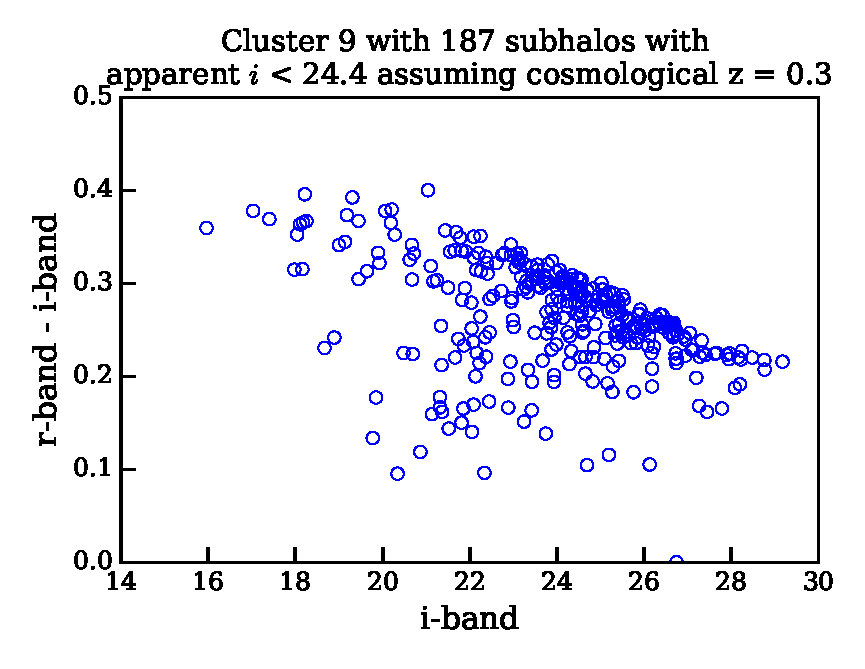
\includegraphics[width=\linewidth]{fig2_color_magnitude_diagram9.eps}
	\caption{Color-magnitude diagram of one of the galaxy clusters that is selected for 
		analysis. This cluster is the 9th most massive. 
		The apparent magnitude is calculated assuming that 
		the cosmological redshift (distance) is $z = 0.3$. 
		We can see a clear overdense region that corresponds to a red-sequence.
		The color-magnitude diagrams of the other clusters can be found in the
		Jupyter notebook at \href{https://github.com/karenyyng/galaxy_DM_offset/blob/master/code/analyses/fig2_color_magnitude_diagram.ipynb}{https://goo.gl/TJmI6s}.
		\label{fig:color_magnitude_diagram}
	} 
\end{figure}

\subsection{Cluster properties}
\label{subsec:cluster_properties}
\subsubsection{Relaxedness of the galaxy clusters}
\label{subsubsec:relaxedness}

Clusters undergo merger activities of a large range of physical scales and 
in the time scale of million of years. 
The dynamical history, or what we call ``non-relaxedness" is hard to retrieve from 
simulations across different saved states and is missing from observations.
We quantify the state of the cluster by providing several quantitative
definitions of non-relaxedness and see how they correlate with $\Delta s$.
Some possible definition of non-relaxedness referred by the simulation community
include:
\begin{itemize}
	\item the ratio of mass outside the dominant dark matter halo over the total mass
		of the galaxy cluster. The lower the ratio, the less substructures there
		are in the cluster. 
	\item the distance between the most bound particle from the center of mass as a
		function of $R_{200c}$. The smaller the distance, there are less asymmetric 
		substructures. 
	\item [TODO] velocity dispersion from selected galaxies those selection
		criteria will be explained in  
\end{itemize}
which are computable from the Illustris data. 
To relate these simulation quantities, we compute more observation oriented 
quantities in the method section \ref{subsubsec:KDE}. 

The Pearson product-moment correlation coefficient
(aka Pearson's r) of the first
two relaxedness criteria for the 43 selected clusters is as high as 0.82. 

\subsection{Selection of the field-of-view}
\label{sec:FOV}

\begin{table*}
\begin{center}
\begin{minipage}{180mm} 
	\caption{ Selection criteria for stellar subhalos (member galaxies) for each
		cluster / group 
\label{tab:member_galaxy_selections}} 
	\begin{tabular}{@{}lcccc@{}}
\hline 
Data &  Selection strategy  & Sensitivity & Relevant section  \\ \hline
Field of view (FOV) & FoF halo finder& comparable to FOV of the Subaru
Suprime camera & \ref{sec:FOV}  \\ 
Observed filter & $i$-band & consistent among the redder $r, i, z$ bands &   
\ref{subsec:galaxy_properties}
\\ 
Cluster richness  & $i \leq 24.4$ and $z = 0.3$  & sensitive to
the assumed cosmological redshift of cluster and & \ref{sec:illustris_sim} \\ 
& & the assumed limiting magnitude of telescope &   \\
Two-dimensional projections & even HEALPix samples over half a sphere &
discussed as results  & \ref{subsubsec:projections}\\  
\hline
\end{tabular} 
\footnotesize{
}
\end{minipage}
\end{center} 
\end{table*}

We make use of the {\bf \texttt{SUBFIND}} member particle for the DM and the 
{\bf \texttt{FoF}} subhalo identification as our
default volume selection scheme for each cluster / group.
We understand that this choice of volume selection can be more ideal than
observational conditions. We make use of this volume selection scheme
for baseline comparisons. 

Assuming a conservative line-of-sight (los) distance 
, i.e. cosmological redshift, with [TODO] $z = 0.4$, 
the projected extent for most of the Illustris galaxy clusters and groups, 
fits inside the field of view of telescopes, such as the Subaru Suprime Camera,
which covers a physical area of [TODO] $\sim 9$ Mpc $\times 7$ Mpc 
(See \href{https://goo.gl/ClZNvM}{https://goo.gl/ClZNvM} for a Jupyter notebook 
showing the extent of the Dark Matter distribution of the most massive 129
clusters).

\subsubsection{Spatial Projections}
\label{subsubsec:projections}
Unlike in staged simulation, picking out a particular projection for a cluster 
does not always make physical sense.
For highly symmetrical clusters, most projections are similar. 
However, for mergers or asymmetrical clusters, 
there is no obvious choice for the plane of projection that can allow us to
understand the cluster. There is no simplistic merger axis that should be 
projected along the plane of the field of view due to possible 3D spiraling
trajectories of the merging components. 

We therefore compute observables based on even sampling of angular orientation 
as our line-of-sight.
As the order of projecting the data and estimating the summary statistic is
non-commutative, we first project the data before estimating any projected 
observable. 
The computation of even angular orientation 
is done by using HealPy, which is a Python wrapper for
{\bf \texttt{HEALPix}} \footnote{HEALPix is
currently hosted at http://healpix.sourceforge.net}
\citep{Gorski2005}. Each line-of-sight centers on a {\bf \texttt{HEALPix}} 
pixel.
% The viewing angles of the projections are defined by an elevation angle
% $\xi$ and an azimuthal angle $\phi$. 
The number of projections that we employed is 768 for each cluster.
Even though there are at least 2 identical projections for each cluster due to
one possible line-of-sight from the front and one from the back, it does not
affect any summary statistic. We do not remove the duplication as it breaks
the rotational symmetry in the 2D plane when we try to compute the 2D population
distribution of offsets.  
Details of the implementation of the projection is available in Appendix
\ref{app:projections}.


\subsection{Properties of the galaxies in Illustris clusters}
\label{subsec:galaxy_properties}

Different galaxies have different masses, so they should not be considered with equal
importance for peak identification, which requires summing
the mass proxies of different galaxies. A comparison of the projected 
DM map, the luminosity map and the number density map of 129 clusters 
can be found at \href{https://goo.gl/kZUWrg}{https://goo.gl/kZUWrg}, 
\href{https://goo.gl/R7VNi9}{https://goo.gl/R7VNi9} and
\href{https://goo.gl/lmQUPd}{https://goo.gl/lmQUPd} respectively.
It is clear from the comparison that the luminosity maps computed from the KDE 
trace the DM distribution more closely than the number density maps. 

One of the most common weighting schemes employed for galaxy data is to weight
by the luminosity in a particular band. We make use of the $i-$band magnitude
associated with each subhalo as the weight. Since the $i-$band is
one of the redder bands, the mass-to-light ratio is not skewed as much due to star
formation activities. 
We further examined if the colors distribution of galaxies in Illustris-1 are
similar to the observed color-magnitude diagrams for clusters.
The Illustris cluster galaxies are realistic enough that it is easy to
identify an overdense region of galaxies known as the red-sequence in the 
color-magnitude diagram such as Fig.
\ref{fig:color_magnitude_diagram}. The red-sequence is prominent even if we
use other colors formed by different combinations of the $r, i, z$ bands.

\section{METHODS}\label{sec:methods}
A common and the most precise way of summarizing the DM distribution in a
galaxy cluster is by finding the lensing peaks 
(\citealt{Medezinski2013}, \citealt{Markevitch2004}, \citealt{Zitrin13}).
Additionally, the peak region is physically 
interesting due to the higher particle density and interaction rates. 
The most direct analogous statistic for summarizing the member galaxy
population in a cluster is therefore, also the peak. 
Comparing the DM peak with the summary statistics of the galaxy population that
are not the peak therefore can have an {\it offset} purely due to the difference in
the choice of the statistic for summarizing the two sets of identically
distributed data. 
We compare four common point statistic or location for summarizing 
the member galaxy population in a galaxy cluster:
\begin{enumerate}
\item Weighted centroids
\item Weighted density peak via density estimate  
\item Shrinking aperture estimate
\item Brightest cluster galaxy (BCG)
\end{enumerate}

We avoid any manual methods for
comparison purposes, scalability and reproducibility. 
Since all the methods listed in this
paper are automated with the source code openly available, 
it is possible for future studies to reuse our code for comparisons. 
% There are a number of decisions ($\sim $[TODO] ADD NUMBER) that one needs to make to 
% determine the summary statistics. We will try to address the sensitivity of the offset
% due to each decision. 
Furthermore, a major advantage for automation is that it allows us  
to apply
the same methods across the different snapshots of the (Illustris) simulations to
examine the variability of $\Delta s$ across time. 


\subsubsection{Computing the weighted centroid}
\label{subsubsec:weighted_centroid}
We follow the usual definition of the weighted centroid is just: 
\begin{equation}
	\bar{\bf x}_w = \frac{\sum_i w_i \vec{x}_i}{\sum_i w_i},
\end{equation}
with $\vec{x}_i$ being the positional vector of each subhalo 
and we use the $i$-band luminosity 
as the weight $w_i$ for the $i$-th galaxy.
Centroids can be biased 1) by subcomponents from merging activities yet the
centroid estimate do not provide explicit evidence for ongoing merger or 
accretion. These estimates are also sensitive to odd boundaries 
of the field of view.

\subsubsection{Cross-validated Kernel Density Estimation (KDE) and the peak finder} 
\label{subsubsec:KDE}
Finding the exact peak of a sets of data points 
involves computing the density estimate of the data points and sorting through
the density estimates. A specific version of this density estimation process is
known as histogramming. During the making of histogram, each data point is
given some weight using a tophat kernel and the weights are summed up at
specific data locations (e.g. $\bf{x}_i$). 
Histogram is not good for peak estimate for {\it sparse} data for two reasons: 1) the
choice of laying down the bin boundaries affects the count in each bin, 2) the choice of
bin width also affects the count in the bin. Only when the available number of data points
for binning is large, the estimates of histograms and smoothed density
estimates are approximately the same. The number of member galaxies ($< 500$) 
is sparse enough for the uncertainty introduced by histogramming to bias our
peak estimate. For the density estimate of galaxy luminosity, 
we adopt a Gaussian kernel. 
The exact choice of the functional form of the smoothing kernel does
not dominate the density estimate as long as the chosen kernel is
smooth \citep{Feigelson2014}. 

The most important parameter of computing the density estimate is the bandwidth
 of the smoothing kernel, which takes the form of a matrix in the 2D case. 
 We illustrate the choice of kernel width with Fig.
\ref{fig:bias_variance_tradeoff}. When the kernel width is
too large (bottom left panel), the data is over-smoothed, 
resulting in a bias of the peak estimate. On the other hand, when the kernel
width is too small, it results in high variances of the estimate and result in
too many peaks due to noise. The decision of having to balance between creating high
bias or high variance estimates is also known as the bias-variance tradeoff. 

\begin{figure*}
	% \includegraphics[width=\linewidth]{figN_mass_richness.eps}
	\caption{This figure is adapted from \citealt{Vanderplas2012} from
\href{http://www.astroml.org/book\_figures/chapter6/fig\_hist\_to\_kernel.html}{http://www.astroml.org/book\_figures/chapter6/fig\_hist\_to\_kernel.html}
under the fair use of the BSD license. \label{fig:bias_variance_tradeoff} }
\end{figure*}
A well-known way to minimize the fitting error from the density estimate is through
a data-based approach called cross-validation to obtain 
the optimal 2D smoothing
bandwidth matrix ($\Hmat$) of the 2D Gaussian kernel for the
density estimate $\hat{f}$:
\begin{align}
	\hat{f}(\chi; \Hmat) &= \frac{1}{n} \frac{1}{(2\pi)^{d/2}|\Hmat|^{1/2}}
	\sum_{i=1}^n w_i \exp((\chi-{\bf x}_i)^T H^{-1} (\chi-{\bf x}_i)),
	\label{eq:cross_validated_bandwidth}
\end{align}
where the dimensionality is $d=2$ for our projected quantities,
$\chi$ represents the uniform grid points for evaluation, and 
$\bf{x}_i$ contains the spatial coordinates for each of the identified member 
galaxies that survived our brightness cut and $w_i$ is again the $i-$band
luminosity weights for each galaxy.
The idea behind cross-validation is to leave a small fraction of data point 
out as the test set, and use the rest of the data points as 
the training set for computing the estimated density.
Then it is possible to minimize the asymptotic mean-integrated squared error
(AMISE)  by searching
for the best set of bandwidth matrix values, eliminating any free parameter. 

Specifically, we made use of the smoothed-cross validation \citep{Hall1992} 
bandwidth selector in the statistical package {\bf \texttt{ks}} \citep{Duong2007} 
in the {\bf \texttt{R}} statistical computing environment \citep{R_core}. 
Among all the different {\bf \texttt{R}} packages, {\bf \texttt{ks}} is the
only package capable of handling the magnitude weights of the data points 
while inferring the density estimates \citep{Deng2011}. 
Although the particular implementation of KDE has a computational runtime of $O(n^2)$, 
the number of cluster galaxies is
small enough for this method to finish quickly ($\lesssim 2$ second per
projection per cluster). 

After obtaining the KDE estimate, we employed both a first and second-order  
finite differencing algorithm to find the local maxima.  
The local maxima were then sorted according to the KDE density in a descending
fashion before we perform peak matching and compute the offset. The exact
procedure is discussed in section \ref{subsec:offsets}. 

For each projection of each cluster, we normalize the density of all significant 
luminosity peaks to those of the brightest peak. 
Then we sum the density of all the peaks for a cluster and call this value
$\nu$. When the value of $\nu$ gets bigger than 1, it indicates the presence 
of projected substructures for that particular projection.

\subsubsection{Shrinking aperture estimates}

Another popular method among astronomers for finding the peak of a spatial
distribution is what we call the shrinking aperture method.
While we do not endorse this method,
we test if the shrinking aperture method is able to reliably recover the 
peak of the luminosity map.
This method is dependent on the initial diameter and the initial center 
location of the aperture.
This method does not evaluate if the cluster is made up of
several components.
The estimate using the shrinking aperture algorithm can be biased by
substructures. The only way to inform the algorithm about substructures would
be to introduce another parameter to restrict the extent of the aperture, or to
partition the data with another (statistical) algorithm.
Furthermore, the convergence of results of this method is unstable. We use a
convergence criteria of having the aperture distance not change more than 2\% 
between successive iterations as a reference. The actual implementation in
Python can be found at \href{https://goo.gl/nqxJl8}{https://goo.gl/nqxJl8} while
the pseudo-code can be find in Appendix \ref{app:shrink_apert}.

\subsubsection{Brightest Cluster Galaxies (BCG)}
The BCGs are formed by the merger of many smaller
galaxies. The galaxy-cannibalism makes BCGs typically brighter than the rest of 
the cluster galaxy population by several orders of magnitude. 
However, star formation can cause
less massive galaxies to be brighter in the bluer photometric bands.
To avoid star formation from biasing our algorithm for identifying the
BCG, we find the brightest galaxies in redder bands i.e. the $r, i, z$
bands and found that they give consistent results for all selected clusters. 
We used the $i-$band to pick the BCG for the plots and the final results. 

\begin{figure*}
	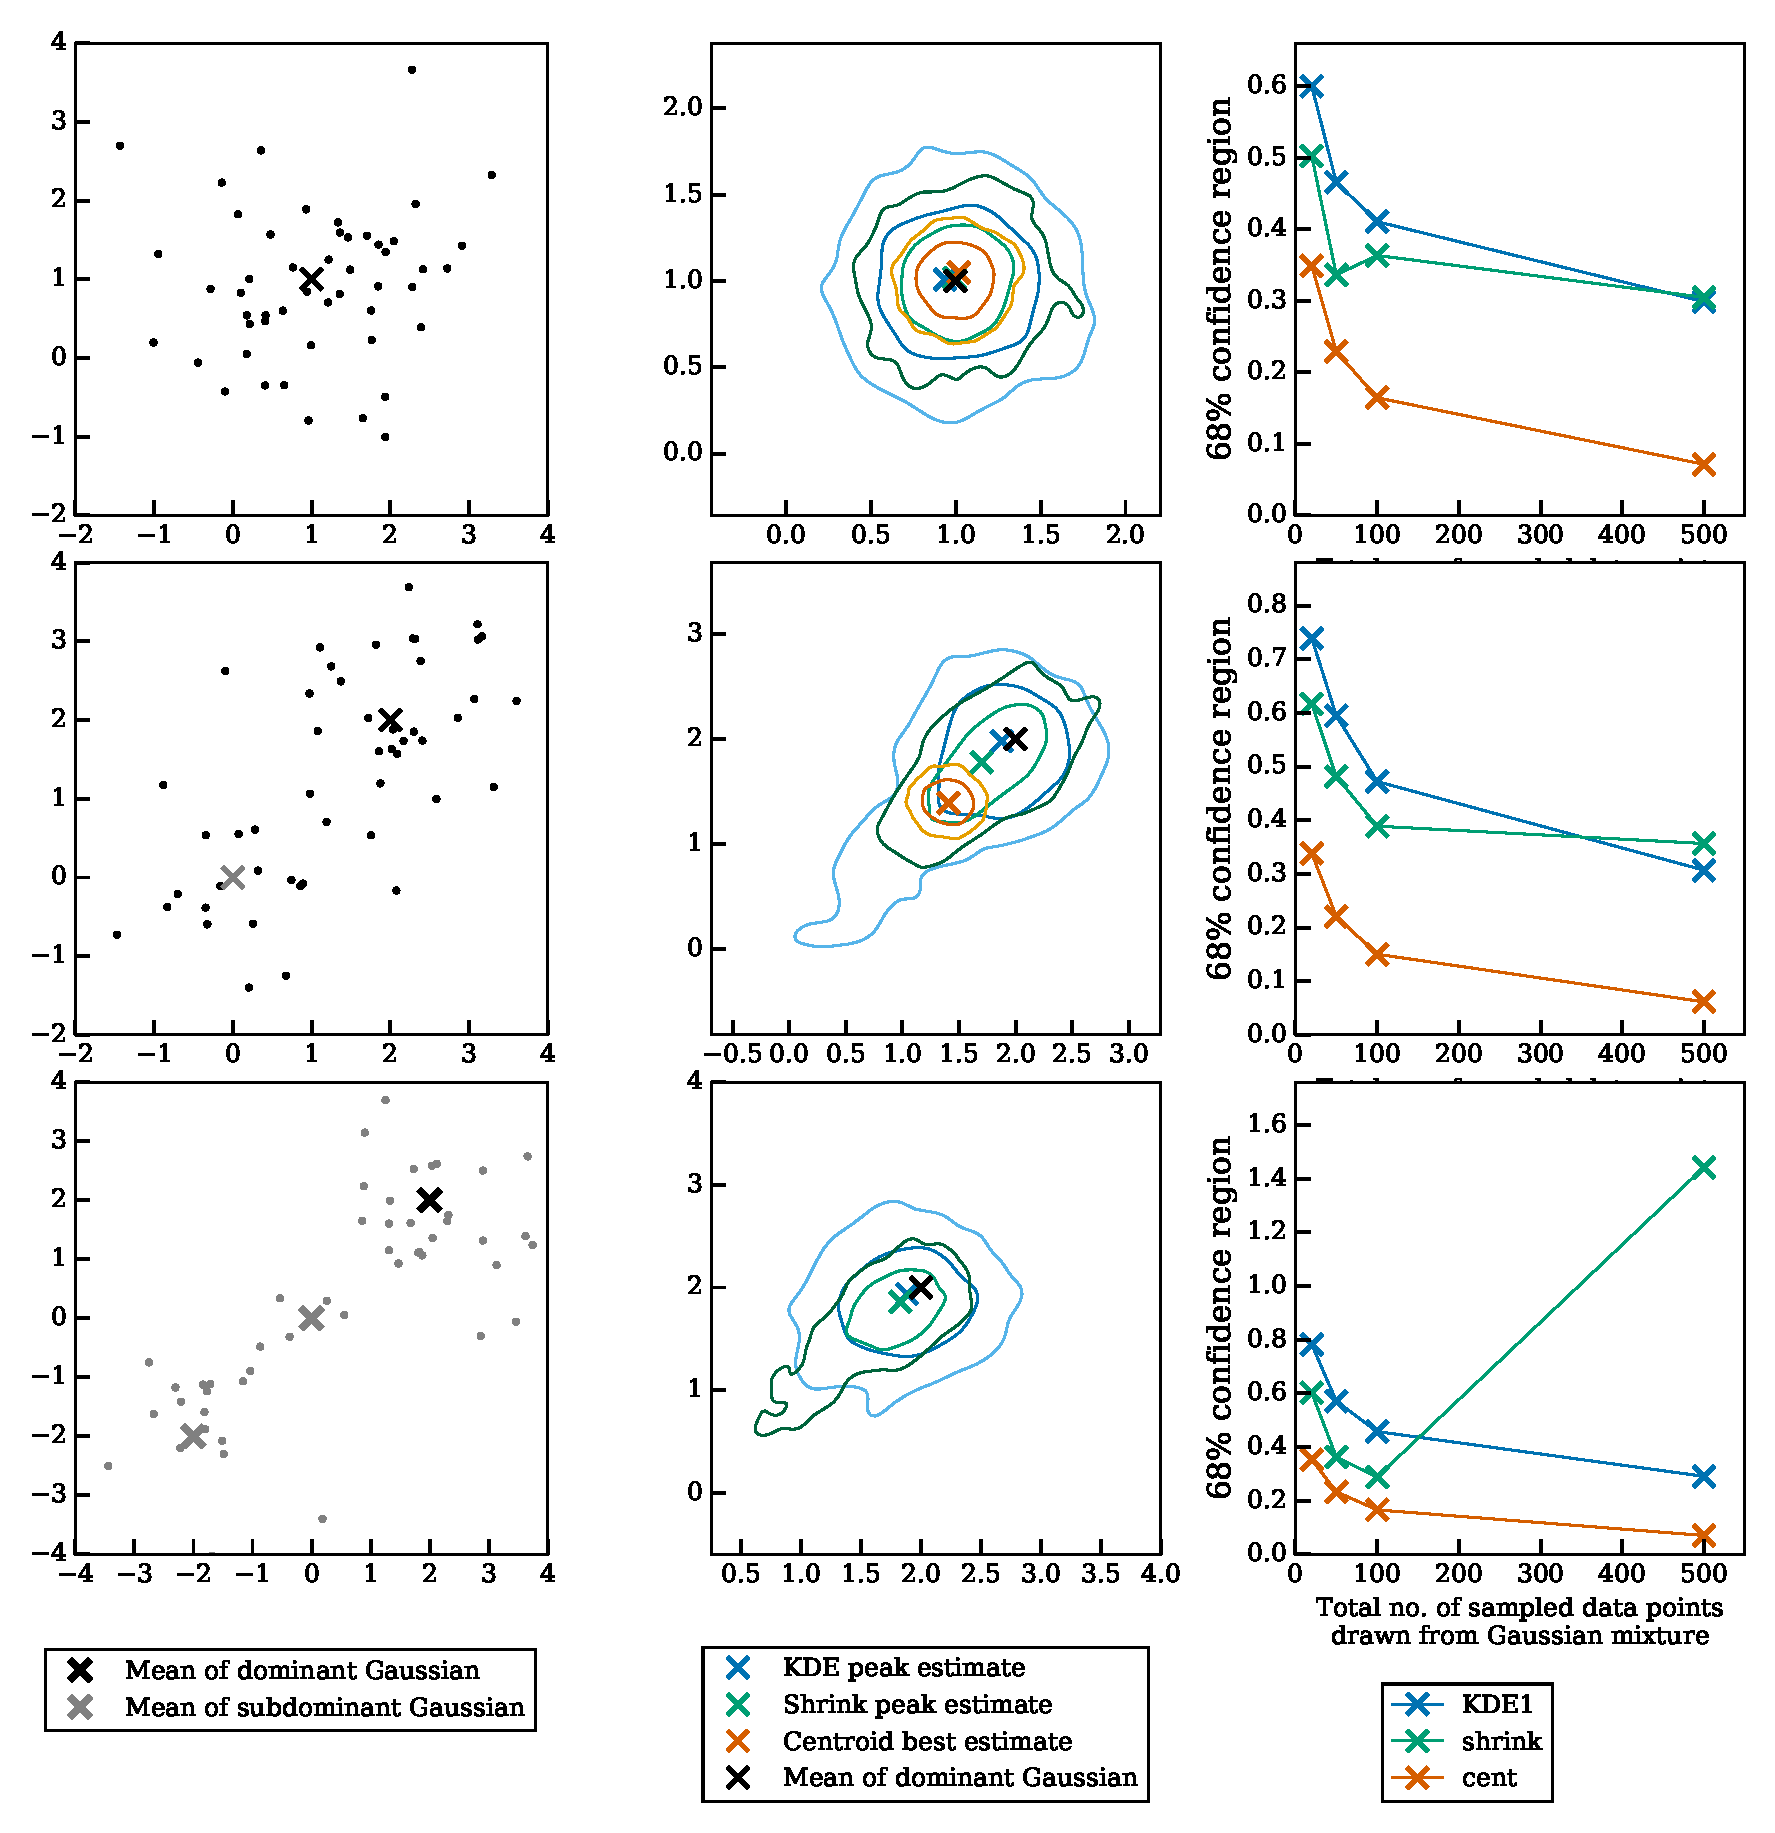
\includegraphics[width=.95\linewidth]{fig3_toy_data_mixtures.eps}
	\caption{Comparison of peak finding performances of different methods by
		drawing data points (i.e. 20, 50, 100, 500) from known number of 
		Gaussian mixtures. 
		Panels from the top row contain data drawn from a single Gaussian mixture. The
		panels from the middle row contain data from two 
		 Gaussian mixtures with weight ratio = 7:3. 
	The panels from the bottom row contain data drawn from three Gaussian
	mixtures with weight ratio = 55:35:10. 
	The left column shows how 50 data points drawn from the fixed number of 
	Gaussian mixtures look like. 
	Due to the statistical nature of this exercise, we sampled the data and
	performed the analyses [TODO: state how many times] many times to
	create the 68\% and 95\% Monte Carlo confidence contours of the estimates in the
	zoomed-in view of the data in the middle
	column. The rightmost column shows how the size (median contour radius) 
	of the confidence regions vary as a
	function of the number of drawn data points from the Gaussian mixtures. 
	From the middle and the rightmost
	column, we can tell that the KDE peak estimate is the most accurate. [TODO] 
		\label{fig:toy_data_mixtures}}
\end{figure*}



\subsection{Comparison of the methods from Gaussian mixture data}
In order to examine the statistical properties of commonly used point-
estimates of the distribution of the galaxy data, we test them on data drawn 
from Gaussian mixtures with known mean and variance. (See Fig.
\ref{fig:toy_data_mixtures}). The main factors that affect the performance of 
the methods are sensitive to the statistical fluctuations of the drawn data, 
e.g. the
spatial distribution of the data, including 1) the density profile and 2) the
location(s) of subdominant mixtures,
, and 3) the number of data points that we draw.
It is also not enough to just
compare the performance by applying each method for one realization of the
data. We provide the 68\% and the 95\% confidence regions by applying the
each method for many Monte Carlo realizations.
In general, the peaks identified from the KDE density is closer to the 
peak of the dominant mixture (more accurate) than 
both the weighted centroid method and the shrinking aperture method.
For example, in the bottom middle panel, it is clear that the green contours
that represents the confidence region for the shrinking aperture peak is
biased due to the substructure, whereas the confidence region for the centroid 
is so biased that it is
outside the field of view of that panel.
For the bottom right plot, there is also a catastrophic outlier for the shrinking 
aperture method for 500 data
points. The outlier shows how the shrinking aperture method can have
radical behavior when there are subclusters in the data.	

\subsection{Modeling the DM map in Illustris-1 and the lensing kernel}
The most well established method of inferring the projected dark matter spatial 
distribution from observations is through gravitational lensing.
It works by detecting subtle image distortions of background galaxies due to
the foreground dark matter. The resolution of the inferred map therefore 
depends on the properties of the source galaxies that are being lensed, 
such as the projected number density, 
intrinsic ellipticities and morphology etc.
To achieve a sufficient signal-to-noise ratio for lensing, 
\citealt{Hoag2016}  has performed simulation for inferring the optimal size
for a Gaussian smoothing kernel for the cluster MACSJ0416. 
In the strong lensing regime, \cite{Hoag2016} found a resolution of 11 arcseconds
can best fit the data. This kernel translates to a physical size of 50 
kpc assuming a cosmological redshift of $z \approx 0.3$.
To compute a DM spatial distribution, we first make histogram with 2 kpc
$\times$ 2 kpc bin size which is larger than the DM softening length of 1.4 kpc. 
After that, we use a Gaussian smoothing kernel of the DM histogram Illustris DM
particle data. We do not perform a cross-validated KDE that has
$O(n^2)$ runtime on the DM data because the
number of DM particles for each cluster is of 
[TODO double check] the order of millions. The DM
resolution is high enough for the histograms to be accurate.  
Physically, the histograms of the dark matter of each cluster 
is analogous to a convergence map from a lensing analysis. 


\subsection{Finding the offsets} \label{subsec:offsets}
It is possible to have several peak estimates from the KDE of the member galaxy 
population of a cluster. 
From the density estimate at each peak, we can sort 
the peaks according to their densities. We only match make use of luminosity 
peaks that are at 
least 20\% as dense as the brightest galaxy-luminosity peak to avoid 
computing the offsets of spurious substructures, such as the peaks due to 
small number of galaxies that are located far away from the main concentration of mass.

In general, there are many more DM peaks because there are many more dark 
subhalos than galaxies for each cluster and the resolution of the DM data is
much higher. To find the nearest match to the significant galaxy peaks,  
we construct a k-dimensional tree (KD-Tree; in our case, k = 2) 
using the densest $n_{\rm DM}$  number of DM peaks:
\begin{equation}
	n_{\rm DM} = \begin{cases}		
		3 \times (n_{gal} + 1) & {\rm if~} n_{gal} < 3 \\
	3 \times n_{gal}  & {\rm if~} n_{gal} \geq 3.
	\end{cases}
	\label{eq:peak_threshold}
\end{equation}
where $n_{gal}$ is the number of significant galaxy peak, and $n_{\rm DM}$
is the number of peaks that went into the construction of the KD-tree.
When there are more
than one dense galaxy peaks located far away from one another, 
the top few densest DM peaks (subhalos) 
can be located around the same galaxy peak.
i.e. there is no one-to-one matching between the luminosity of galaxies and the
density of detected DM peaks.
Matching purely based on density and luminosity leads to larger offsets.
From inspection, using eq. (\ref{eq:peak_threshold}) works well to match the 
appropriate peaks.  After identifying the DM peaks, we also compute the 
offsets 
between the DM peaks, and the following spatial estimates, including 
1) the most bound particle 
2) the shrinking aperture peaks, 
3) the number density peaks, 
4) the BCGs, and
5) the luminosity weighted centroid.

Since there can be more than one number density peak from the corresponding KDE
map, we also use a KDE tree to location the closest peak to the identified DM
peak.

[TODO] Figure out how the Illustris simulation figure out the most bound 
particle.
The most bound particle is the location with minimum 
gravitational potential of the {\bf \texttt{Subfind}} identified cluster.
Due to substructures, it is possible for there to be several minima of similar 
gravitational potential level. 

\subsection{Constructing the non-parametric hypothesis test} 

After matching the peaks, we use the offsets as the basis of our 
non-parametric hypothesis test. 
We compute the p-value as the highest density interval of simulated offsets 
that are below observed values of 
offsets in the literature.  
This gives us a rough estimation of the probability 
of seeing the offset from real observations under the null hypothesis of CDM 
being true. We also provide some robust statistic characterizing the 
distribution of offsets computed from each of the listed methods.

The different representations of $\Delta s$ have different statistical power
for the hypothesis test, i.e. the spread of the offset distribution in
different representation differ so
it affects the significance of an observation. 
The most faithful representation of the offsets without any information loss
is:
\begin{equation}
	\Delta {\bf s} = ({\bf x}_{\rm gal} - {\bf x}_{\rm DM}, 
	{\bf y}_{\rm gal} - {\bf y}_{\rm DM} ).
	\label{eq:2D_offsets}
\end{equation}
The PDF in \ref{eq:2D_offsets} peaks at (0, 0) when there is no real offset.
However, when one takes the magnitude of $\Delta {\bf s}$, i.e.:
\begin{equation}
	|\Delta {\bf s}| = \sqrt{({\bf x}_{\rm gal} - {\bf x}_{\rm DM})^2 + 
	({\bf y}_{\rm gal} - {\bf y}_{\rm DM})^2},
	\label{eq:magnitude_offsets}
\end{equation}
the resulting 1D distribution of $|\Delta {\bf s}|$, 
those support being [0, $\infty$),
will not peak at zero even if the original
distribution of $\Delta {\bf s}$ peaks at (0, 0). On the other hand, 
the 1D distributions along a particular spatial axis, e.g. $\Delta {\bf x}$ and $\Delta {\bf y}$,
each with a support of $\mathbb{R}$, will not exhibit a discontinuity when
the offset is zero. 

Due to the caveat of representing the offset as $|\Delta {\bf s}|$
and the completely asymmetric distribution of $|\Delta {\bf s}|$
, we compute the hypothesis test significance level with the 
 offset $\Delta {\bf x}$ along one of the spatial axes.
We also provide a table of statistic of different ways of representing the
offsets.

\section{RESULTS} 
\label{sec:results}

\subsection{Offset between galaxy summary statistic and the most bound particle}

As a sanity check, we computed the offsets between different galaxy summary
statistic and the most gravitationally bound particle (aka most bound particle). 
The ranking in terms of increasing distance 
to the most bound particle computed by different method is as follows:
\begin{itemize}
	\item BCG 
	\item densest peak of the luminosity map created by weighted the KDE 
		\item shrinking aperture center from the luminosity weighted galaxy data
		\item densest peak of the number density map created by the unweighted KDE 
\end{itemize}

The table denoting the exact distribution of offsets from the most bound 
particle is available in Appendix [TODO]. 
In fact, most of the BCG offsets are very small except for two clusters with ID 13
and 33. Both clusters have all the values  of $\nu > 0 $ over different projections  
and from the projected visualization, we confirm that
both clusters have significant substructures. It is therefore possible for the
most bound particle to have similar gravitational potential level as another 
substructure where the BCG is located. 

\begin{table*}
	\begin{minipage}{170mm}
	\begin{center}
		\caption{Robust estimates and the distribution of offsets along the y-axis
			(This is different from the magnitude which has discontinuity at zero).
		\label{tab:p_val_table}
	}
	\begin{tabular}{llccccccc}
\toprule
sample & offset (kpc  &  location &  lower 68\% &  lower 95\% &  lower 99\% &  upper 68\% &  upper 95\% &  upper 99\% \\
\midrule
all $\nu$& $\Delta y_{\rm BCG}$                &         0 &          -3 &         -22 &        -496 &           3 &         456 &        1449 \\
& $\Delta y_{\rm KDE}'$               &         0 &         -25 &         -79 &        -127 &          25 &          79 &         126 \\
& $\Delta y_{\rm num. dens}$          &        0 &         -84 &        -303 &        -693 &          84 &         302 &         691 \\
& $\Delta y_{\rm shrink}'$            &        0 &         -65 &        -295 &        -652 &          65 &         295 &         655 \\
\midrule
$\nu < 1.2$& $\Delta y_{\rm BCG}$              &        0 &          -3 &         -10 &         -19 &           2 &           9 &          19 \\
& $\Delta y_{\rm KDE}'$             &         0 &         -18 &         -48 &         -82 &          18 &          48 &          83 \\
& $\Delta y_{\rm centroid}'$         &        0 &        -108 &        -255 &        -395 &         108 &         254 &         394 \\
& $\Delta y_{\rm num. dens}$        &        0 &         -73 &        -195 &        -303 &          73 &         195 &         302 \\
& $\Delta y_{\rm shrink}'$          &         0 &         -51 &        -187 &        -285 &          51 &         187 &         285 \\
\midrule
$1.2 < \nu < 2.0$& $\Delta y_{\rm BCG}$        &         0 &          -3 &        -172 &        -699 &           4 &         860 &        1597 \\
& $\Delta y_{\rm KDE}'$       &        0 &         -33 &         -90 &        -128 &          33 &          90 &         127 \\
& $\Delta y_{\rm centroid}'$   &         0 &        -266 &        -673 &        -926 &         266 &         673 &         926 \\
& $\Delta y_{\rm num. dens}$  &         0 &         -89 &        -350 &        -776 &          89 &         347 &         776 \\
& $\Delta y_{\rm shrink}'$    &        0 &         -85 &        -385 &        -773 &          85 &         385 &         776 \\
\bottomrule
\end{tabular}

	\end{center}
	\end{minipage}
\end{table*}

% \begin{landscape}
\begin{table*}
	% \begin{minipage}{180mm} 
	 \begin{center}
	 \caption{Observed offsets from bimodal clusters with confirmed major mergers.\label{tab:offset_results}} 
	 \begin{tabular}{@{}lccccccc@{}}
	 \hline 
	 Cluster & $\Delta s$ (kpc) & galaxy peak & DM peak &  p-value & subcluster &
	 mass ($10^{14}$ M$_\odot$) &  reference\\
	 \hline
	 MACS J0025.4-1222 & & & & & southeast &2.5& \citealt{Bradac2008}\\
	 MACS J0025.4-1222 & & & & & northwest &2.6& \citealt{Bradac2008} \\
	 DLSCL J0916.2+2951 & 129 & number density & weak-lensing &  & southern & 3.1 &  \\
	 DLSCL J0916.2+2951 & 47 & number density & weak-lensing &  &northern & 1.7 & \\
	 Abell 520 & & & & & & & \\
	 ACT-CL J0102-4915 & 570 & number density & weak-lensing & & southeast & 11 & \citealt{Jee2014} \\
	 CIZA J2242.8+5301 & $\sim$200 & number and luminosity & weak-lensing & & both
	 subclusters & & \citealt{Jee2015}\\ 
	 \hline
	 \end{tabular} 
	 \end{center} 
	% \begin{minipage}{180mm} 
\end{table*}
% \end{landscape}


\begin{figure*}
	\begin{center}
	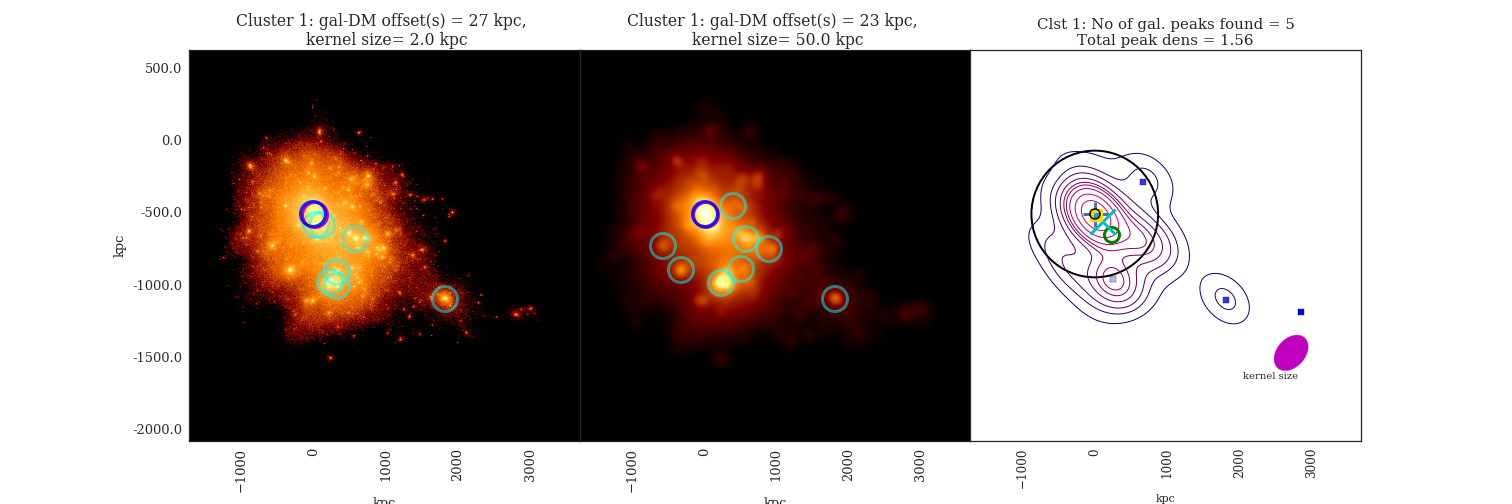
\includegraphics[width=0.85\linewidth]{Fig4_clst1_48_225.png}
	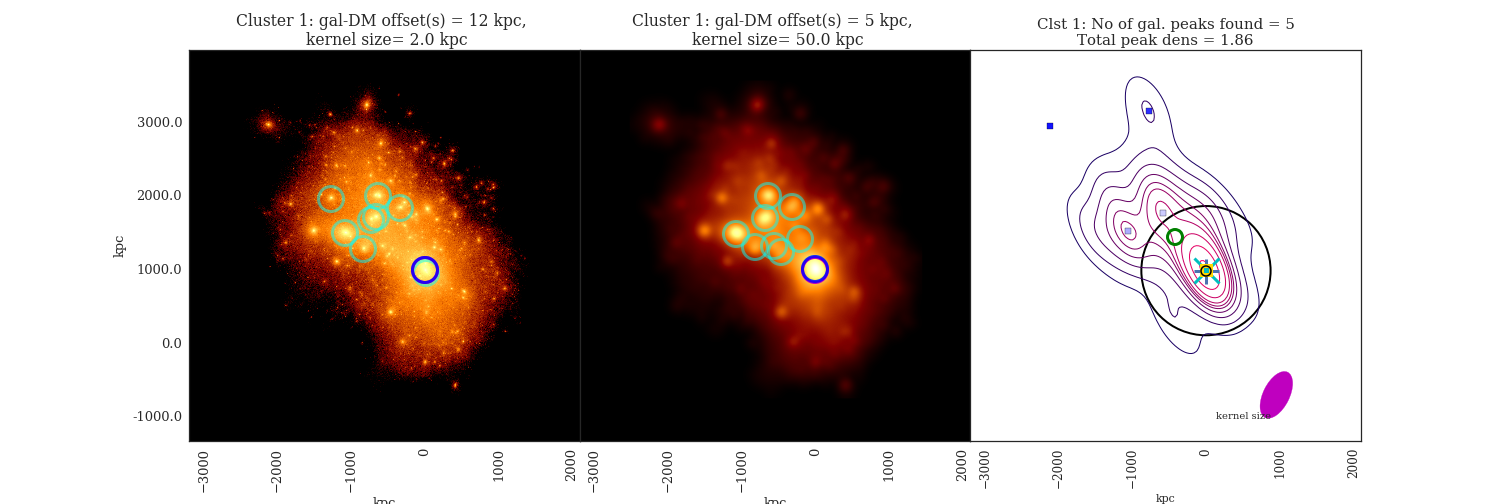
\includegraphics[width=0.85\linewidth]{Fig4_clst1_48_135.png}
	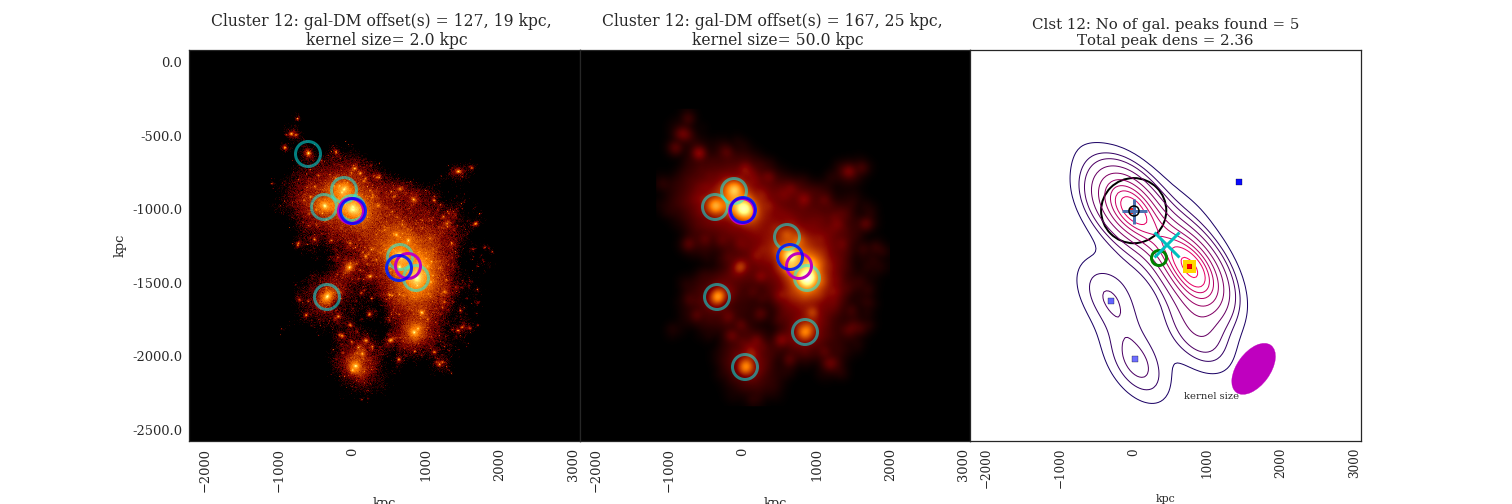
\includegraphics[width=0.85\linewidth]{Fig4_clst12_48_135.png}
	\caption{[TODO merge margin between left and middle panels] 
		Visualization of clusters (each row is for the same projection
		of the same cluster). {\bf Left column:} Projected density distribution of DM	
		particle data (density overlay). 
		The identified density peaks are indicated by colored circles. 
		{\bf Middle column:} The same DM projection but with treated with a 50 
		kpc smoothing kernel (kernel size indicated by white dot on lower right of
		the figure. Note that the thickness of the dot may be larger than 2 kpc
		for the plots on left hand column).
		{\bf Right column:} Projected galaxy kernel density estimates (KDE) of 
		the $i$-band luminosity map for the member
		galaxies of the same clusters. Each colored contour denotes a 10\% drop 
		in density mass starting from the highest level in red. Each of 
		the magenta ellipse on the
		bottom right corner of each plot show the Gaussian kernel matrix 
		$H$ from eq. (\ref{eq:cross_validated_bandwidth}). 
		The big black 
		circle is centered on the most bound particle as identified by {\bf
		\texttt{SUBFIND}} and the radius of the circle indicates the 
		three-dimensional region in
		which the average density is 200 times the critical density of the universe
		(a.k.a. R$_{\rm 200C}$).
		See \href{http://goo.gl/WiDijQ}{http://goo.gl/WiDijQ} 
		and \href{http://goo.gl/89edcM}{http://goo.gl/89edcM} for the 
		visualization of the selected clusters inside two Jupyter notebooks.
		\label{fig:select_peak_visualization}
	}
\end{center}
\end{figure*}


\subsection{Galaxy-DM Offset in Illustris}
% talks about the overview of the offsets in the simulation

\subsubsection{Two-dimensional (2D) offsets}
The 2D distribution of $\Delta s$ from most methods peak at
around zero ($\lesssim 4$ kpc) with rotational symmetry, 
except the luminosity weighted centroid method (See table 
\ref{tab:offset_distributions}).
The spread of $\Delta s$ computed by each method 
differ (See Fig. \ref{fig:offset_distributions} for the distribution along
the y-axis). The offset $\Delta s_{\rm BCG}$ peaks sharply near zero but 
contains outliers. Having outlier is possible 
because the DM peak is chosen as the closest DM peak to match the
brightest luminosity peak in a particular projection.
When there are distantly separated subclusters of similar masses, 
the brightest projected luminosity peak 
may shift from one subcluster to another subcluster between different projections,
while the BCG identification is unchanged between projections.

The offsets computed by the peak from the luminosity weighted KDE 
has the second smallest variance. The 68\% percentile of $\Delta y_{\rm
KDE}'$ is at around $\pm 25$ kpc. Using shrinking aperture to estimate
the peak location from the luminosity map increased the 68-th percentile of the
offset to more than double those of $\Delta y_{\rm KDE}'$ at $\pm 65$ kpc.
The peak estimate from the number density map has even larger variance 
(with its 68-th percentile at $\pm 84$ kpc). 
The spread of the offsets inferred by each method will affect their ability
for constraining $\sigma_{\rm SIDM}$. 

% \subsubsection{Offsets from all clusters}
% From Fig. \ref{fig:offset_distributions} we can tell that there are

% \subsubsection{Offsets from bimodal clusters}


\begin{figure*}
	\begin{center}
	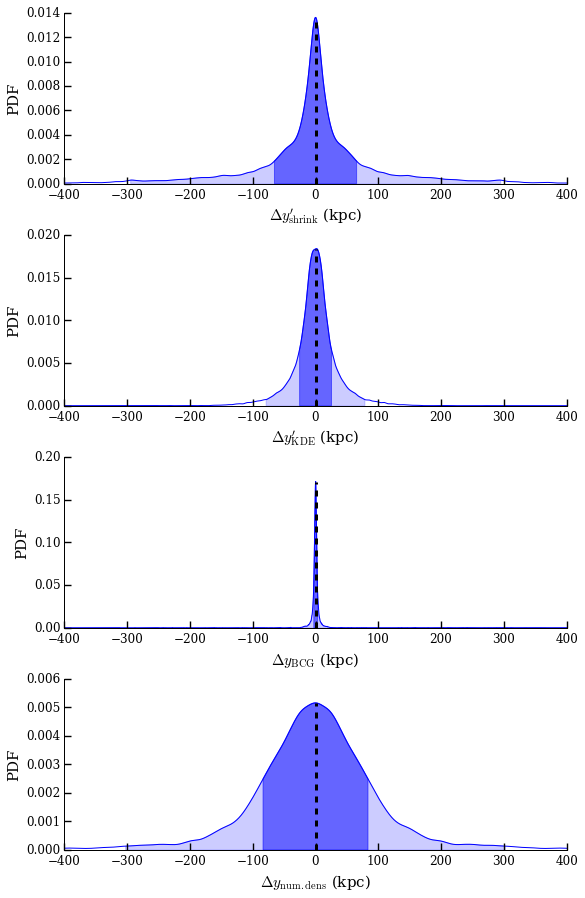
\includegraphics[width=0.65\linewidth]{fig5_symmetrical_1D_pdf.png}
	\caption{ 		
		The distribution of different offsets of 43 clusters with all 768
		projections. For estimates where several peaks of galaxy data are 
		possible, only the densest peak is matched to the DM peak for computing
		the offsets in this figure. 
		The dark blue area indicates the 68\% density interval
		while the light blue area shows the 95\% density interval. 
		The table summarizing the statistic of each distribution is available in
		table 
		\label{fig:offset_distributions}
	}
\end{center}
\end{figure*}

\begin{figure*}
	\begin{center}
	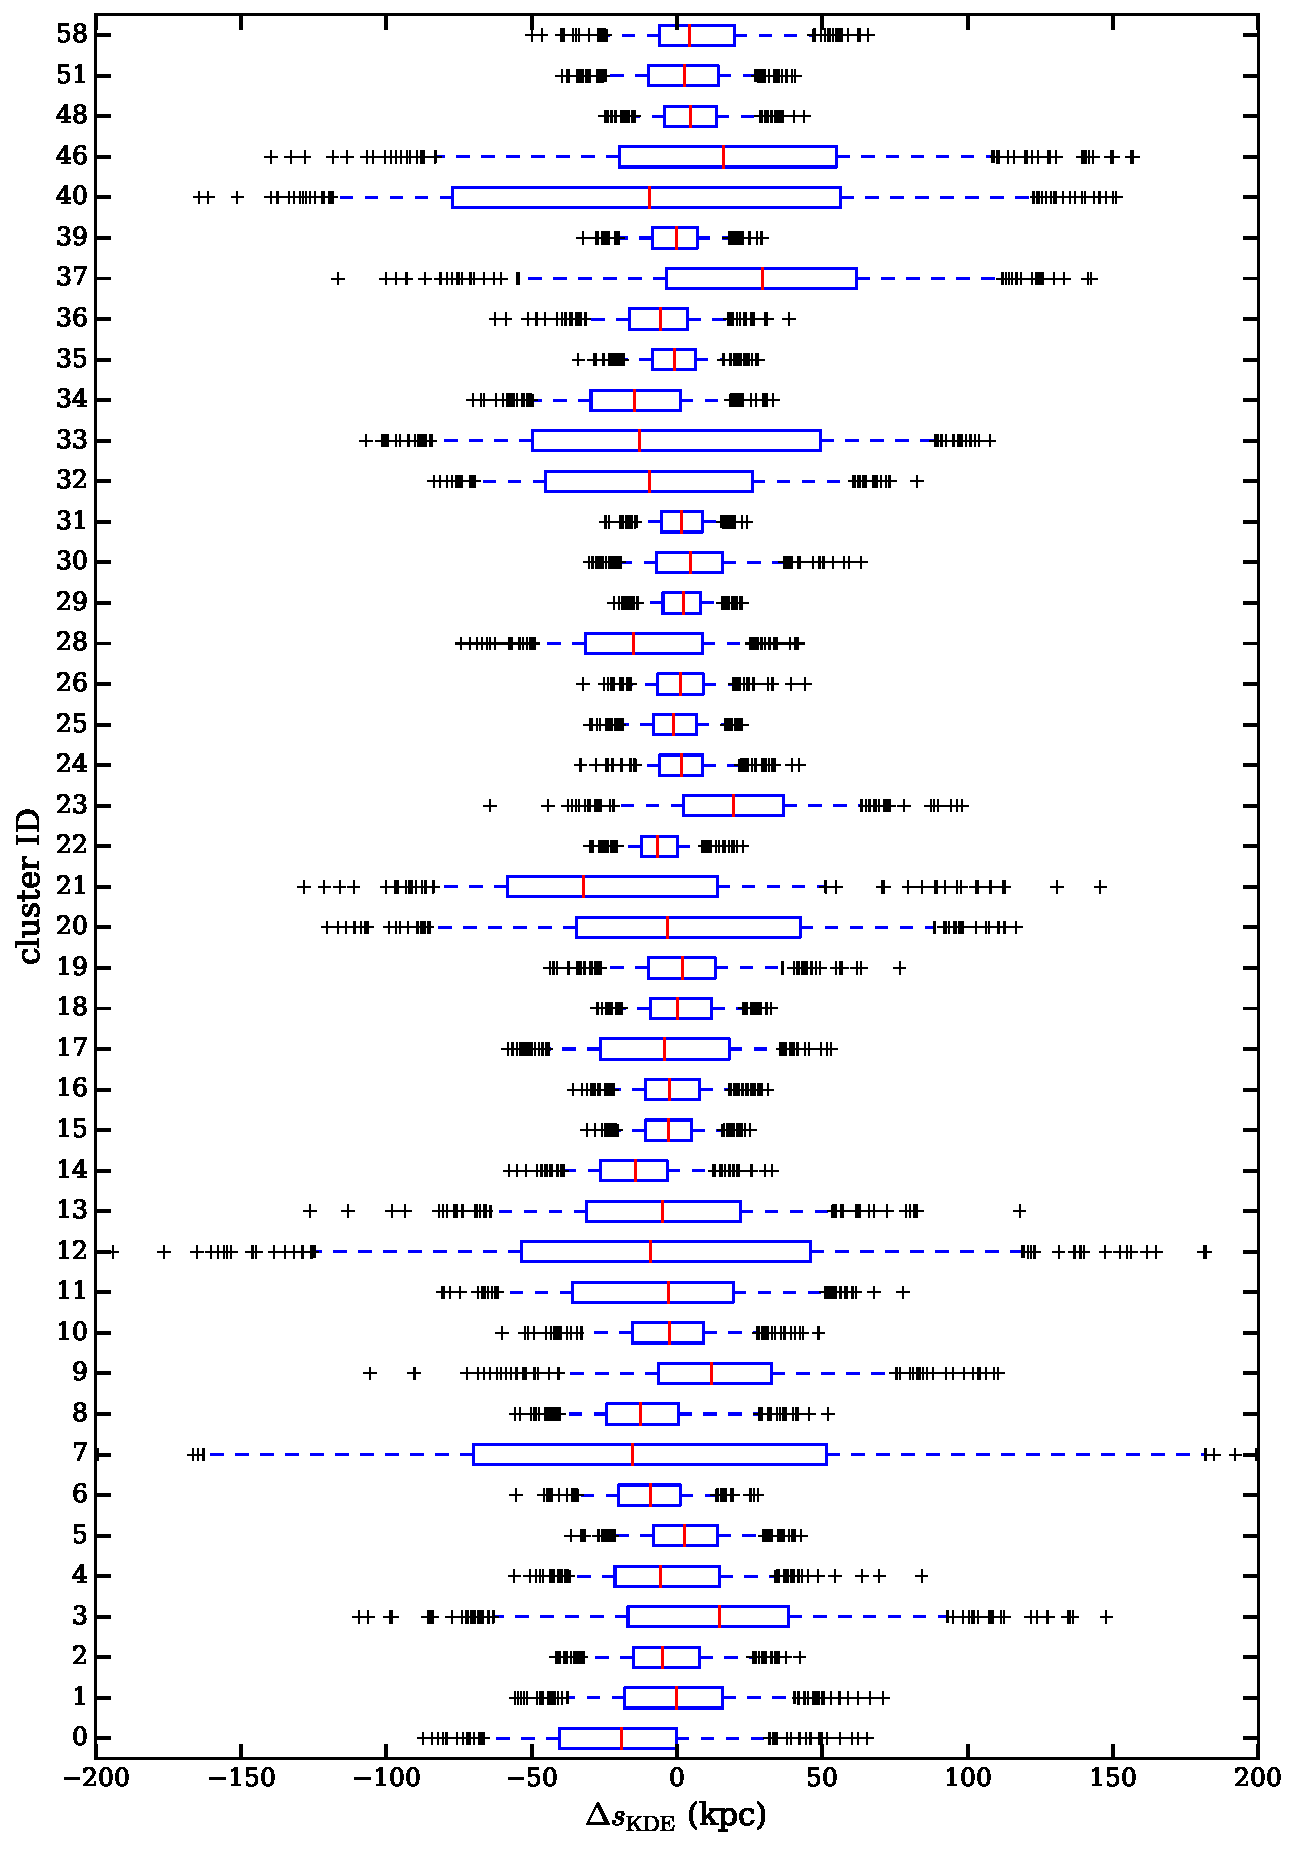
\includegraphics[width=0.85\linewidth]{fig7_projected_KDE_offset_distribution.pdf}
	\caption{A box plot showing the distribution of projected offsets for each cluster 
		based on 768 projections. The red line shows the median of the projections,
		the box encompasses the 25\% and 75\% percentile of the distribution while
		the whiskers mark the 5\% and the 95\% percentile. The other black crosses
		are data points with extreme values beyond the 5\% and 95\% percentile.
		The offsets were computed between the closest DM 
		peak to the brightest luminosity peak of each cluster. 		
		\label{fig:projected_KDE_offset_distribution}
	}
\end{center}
\end{figure*}




\subsection{Offset projection uncertainty of each cluster}
When we gather the offsets $\Delta s_{\rm KDE}'$ of the 
768 projections for each cluster,
we can find the offset uncertainty due to projection effects.
The distribution of $\Delta y_{\rm KDE}'$ of each cluster is illustrated in the
box plot of Fig. 
\ref{fig:projected_KDE_offset_distribution}.
We use a robust statistic, the biweight mid-variance to characterize the spread
of the distribution instead of the standard deviation, which can be more
susceptible to outliers.
The biweight mid-variance of the $\Delta s_{\rm KDE}$ of half of the clusters
is $< 23$ kpc. Only 4 clusters have mid-variance $ > 40$ kpc. 
 
\subsection{Correlations between different variables and the offsets}

Physical quantities that have positive correlation $\sim 0.7$
with the maximum $\Delta s_{\rm KDE}$ of each cluster include the two
non-relaxedness criteria mentioned in section \ref{subsubsec:relaxedness},
There is also very strong correlation of $\sim 0.8$ 
between the two non-relaxedness quantity 
and the median total density of the luminosity peaks $\nu$ of each cluster.
The offset $\Delta s_{\rm KDE}$ also show a high
correlation of 0.77 with $\nu$. 
The FoF mass of clusters shows slight correlation of 0.28 with the median total density
of luminosity peaks $\nu$ of each cluster but no significant correlation (0.14) with
$\Delta s_{\rm KDE}$. 

There is slightly negative correlation ($\sim -0.2$) between the different mass measured within
a certain density threshold, i.e.  $M_{200C}$ and $M_{500C}$, with $\Delta
s_{\rm KDE}$ and $\nu$.  
A lot of the mentioned correlations are consistent with the
measurements of substructures in the cluster. 
Surprisingly, there is no significant correlation between the richness of the
clusters and $\Delta s_{\rm KDE}$ and $\nu$. This may be due to the fact that
the peak estimate is only affected strongly by a few bright galaxies near the
peak.

% We subset the data and visually inspected the samples with the largest 
% galaxy-DM offsets $\Delta s_{\rm KDE}$. We found that ...  
% 
% \subsubsection{Correlations between the offsets and properties of the 
% cluster / groups}
% [TODO] examine the relationship between
% \begin{itemize}
% \item 3D relaxedness
% \item mass 
% \item richness  
% \end{itemize}
 
 
 
\section{DISCUSSION}\label{sec:discussion}

\subsection{Other findings from the visual inspection of the simulated galaxy clusters}
We inspected both the luminosity maps and the
number density maps of the member galaxy populations.
With the same selection of bright galaxies of apparent $i$-band$ < 24.4$ at
$z=0.3$, the luminosity maps in general resemble the DM maps more closely than 
the number density maps.
In real observations, missing selection of member galaxies, or 
foreground objects can both affect the inference of the galaxy spatial 
distribution. The number density map can be less susceptible to bias from bright 
foreground objects. It is less clear about the effect of missing member galaxies 
for computing the luminosity map because there is a selection bias favoring 
bright member galaxies.

% From the high resolution visualization of the DM maps (two-dimensional
% histograms with 2 kpc bins) in 
% Fig. \ref{fig:select_peak_visualization}, we can tell that some clusters clearly
% possess multiple subclusters with visible separations between the subclusters, 
% e.g. cluster 12 visualized on the panels on row 3 of the plot. 
% However, there are also many clusters that contain  
% only one main component but show several closely-located density peaks in the
% densest region. This illustrates why finding a `center' or peak of a cluster 
% is an ill-defined notion. Most of the density-based statistics 
% are only unambiguous for smooth, symmetrical data.  

% 
% Furthermore, we show a lower-resolution visualization of the DM surface
% map in Fig. [TODO] compared to the higher resolution map, we can see a clear
% shift in the peak location. This illustrates that peak / center finding is also
% subject to noise from the data.
% 
% Sometimes when the peaks are mismatched, it is due to a resolution difference 
% between the higher resolution DM data and the sparse galaxy data. 
% (See middle bottom panel in Fig. \ref{fig:select_peak_visualization})
% 
% 
% 
% The main reasons for the existence of several peak estimates include:
% 1) Extended substructures that exist within the cluster, which we call
% subclusters, although the boundaries of subclusters are ill-defined.
% 2) Galaxies that are located further away from the main concentration of mass.
% These peaks are excluded based on density cuts.
% 3) This last case illustrates the difficulty of pinpointing a point-estimate
% such as a `center` . It is 
% possible to have more than one bright galaxies spatially close to the main
% concentration of mass. 
% (See the right most panel of Fig. \ref{fig:select_peak_visualization}
% where the galaxy luminosity peaks are represented with squared markers that are
% colored according to the relative density to the densest galaxy peak of that 
% projection). 
\subsection{Comparison to surveys of relaxed galaxy clusters}
Using X-ray selected relaxed galaxy clusters, 
\citep{George2012a} reported $\Delta s$ the order of 50 kpc to 150 kpc. 

huge offset

galaxy centroid 

\subsection{Comparing the offset distributions with merging cluster observations}

Our estimated distribution present in table \ref{tab:p_val_table}
represents a lower bound of the spread of offsets.
This is due to the high purity and completeness of the Illustris data.
Most observations of massive galaxy clusters with total mass of M$_\odot
\approx 10^{14}$ have richness $\lesssim 300$, while the most massive Illustris
cluster (M$_{\rm FoF} = 3.23 \times 10^{14} M_\odot$) has a richness of 483.
We do not further divide the cluster sample base on the dynamical state because
they are realizations of the possible dynamical states of clusters.
Most of them are relaxed while a small number ($\sim 3$)


If we restrict to comparison of clusters total mass $\sim 10^{14} M_{\odot}$,
there is no clusters with offsets 
that go beyond our reported 95-th percentile interval.  

The largest observed $\Delta s_{\rm num. dens} \approx 570$ 
kpc to date is from El Gordo (ACT-CL J0102-4915; \citealt{Jee2014}). 
And the number density peak in \citep{Jee2014} is determined via a shrinking 
aperture algorithm (via private communication).
The luminosity peak of El Gordo, however, is located much closer 
to the DM peak location of the lensing convergence map.
El Gordo is also more much more massive ($10^{15} M_{\odot}$) than the Illustris
clusters.
Other large $\Delta s$ from mergers are reported at the level of 200 kpc 
using the number density peak of CIZA J2242.8+5301 \citep{Jee2015}
. These offset level are within the 95\% percentile level 
when we look at $\Delta s_{\rm num. dens}$. The reported 
luminosity peak offset $\Delta
s \approx 200$ kpc, however, goes beyond the $99\%$ level of our reported
intervals. CIZA J2242.8+5301 is located close to the plane
of the Milky Way with high chance of star contamination. 
Again, CIZA J2242.8+5301 is more massive (total mass $\sim 10^{15} M_{\odot}$) 
than the Illustris clusters.

% \subsection{The statistical performance of different peak finding methods}
% The difficulty in matching is not necessarily due to wrong algorithms.
% When the substructures of several important physical scales are present due to
% hierarchical clustering, peak finding is not a well defined problem.
% It is possible for a smaller group-sized halo to be embedded in a
% galaxy-cluster size halo, or several group-sized halo have the majority of its
% mass overlapped with another halo.
% There is no unique solution for specifying the physical boundaries of substructures
% before finding the corresponding peaks. 
% While the peak-matching by galaxy-peaks that
% we performed is an ad-hoc approach, only picking spherically-looking can only
% guarantee relaxedness up to a certain extent. 
% The number of non-relaxed clusters far outnumber the ones that are dynamically 
% relaxed. 

\subsection{Comparison to other simulations}
\subsubsection{Comparison to other cosmological simulations}
 
% Assume dynamical equilibrium 

 
\cite{Cui2015} X-ray center, BCG
% 
% does not provide the pairwise offset between the DM and the galaxy distributions
% but rather the offset between the minimum potential and DM. 
% computing the offset from the population statistic of the DM spatial distribution 
% with the population galaxy distribution destroys the possible correlations.
% 
% Fig. 3 in \cite{Cui2015} shows both the DM peak and the galaxy offsets to the 
% minimum gravity potential center but that representation destroys the 
% correlations. 
% gives no p-value for comparison. 
% width of histograms can affect the distribution  
% taking the absolute magnitude of the offset can bias the data  
% \cite{Harvey2013d} consistent with zero offsets using the {\bf
% \texttt{Wavedetect}} wavelet analysis algorithm. 
% Provided nice theoretical motivation for describing how galaxies and DM
% population would behave 
% They have only verified that their model of SIDM work for 
% $\sigma_{\rm SIDM} = 0$ but not any model with $\sigma_{\rm SIDM} > 0$
% 
\subsubsection{Comparison to other staged simulations}
% 
% In this work, we test purely for the offset due to statistical noise and
% missing variables such as projection and impact parameter 
% 
% \cite{Randall2008d} can be thought of a controlled experiment where 
% only the effects of SIDM is in place.
% This is because a large number of tracer galaxies were painted on as 
% collisionless particles, using identical distributions between the galaxies 
% and the DM particles at the beginning of each run. 
% 
% Statistical uncertainties overwhelm the signal of SIDM.
% 
% \cite{Robertson2016}
% 
% 



% [TODO] cite Stacey
% 
% The 
% 
% It is not clear about the ability of $\Delta s_{\rm SIDM}$ for differentiating 
% between different $\sigma_{\rm SIDM}$ models. 
% 
% It is unclear that $\Delta s$ is a sensitive observable to signatures of
% $SIDM$.
% 
% 
% At $\sigma_{\rm SIDM} \approx 1.25 $cm$^2$ / g, 
% \citealt{Randall2008d}, \citealt{Robertson2016} only found an offset of $50
% kpc$, this is completely within the population uncertainties of offsets, 
% while the projection uncertainty of a cluster can be as large as  
% [TODO]$ $ kpc.
% 
% 
% Bullet cluster 
% 
% 
% \subsubsection{Estimation of the SIDM cross section from the Illustris offsets}
% Since the Illustris simulation assumes CDM, it is interesting to see if we can
% infer any non-zero $\sigma_{\rm SIDM}$ from the offset estimates based on
% different methods.  
% 
% 
% 
% 

\subsection{Comparison to other observational studies}

Caution when comparing to observational studies.



With high completeness and purity of member galaxy data, 
luminosity peaks  


\subsection{Offset between the BCG and the DM peak}
 
\cite{Zitrin2012}
\cite{Zitrin2012a}
\cite{Mohammed2014}
miscentering lensing peak for stacking weak lensed signal from clusters.  

Centering is not a well posed problem when there are multiple dense subhalos in the densest
region of a cluster.

The problem is easier when the dense subhalos are spaced below observation resolution. 
However, when the dense subhalos are spaced within 50 kpc of each other in
comoving units.  

Unfortunate reliance of outliers of offset distribution to detect signal 
scrutiny of their parameter choices for the inference spatial distribution 

% 
% Weak lensing observations infer mass distribution of both baryonic and dark matter.   
% 
% Central galaxy paradigm (CGP)
% \begin{itemize}
% 	\item \cite{Ford2014} paper about miscentering in CFHT 	
% 	\item \cite{George2012a} about miscentering
% \end{itemize}
% 
% 
% 
% 
% 
% % As there are no well-established procedure for summarizing the peak or the
% % center of a cluster, nor there is a good  
% There are many aspects of the analysis that is not covered by this study that
% are performed for analyzing observational data, such as 
% 
% \begin{itemize}
% 		\item galaxy membership identification along the line of sight
% 		\item removal of foreground galaxies  
% 	\end{itemize}
% 	that are important for calculating the $\sigma_{\rm SIDM}$ with using a
% 	galaxy-DM offset. 
% 
% 
% \subsection{Galaxy-DM Offset in observations of Merging Galaxy Clusters}
% how the offsets will translate to a $\sigma_{\rm SIDM}$.
% 
% 
% \subsection{How to use $\Delta s$ to constrain $\sigma_{\rm SIDM}$}
% 
Statistical aspects that one should take into account when constructing such a
test include: 
\begin{itemize}
\item whether the population PDF of offsets have converged  
\end{itemize}
% 
% 
Characterizing the state of the cluster is not trivial.
% Although in such a high dimensional 
% % 
% 
% When there are real observations that lie sufficiently far away from the 95\% 
% confidence region of the population distribution of the Illustris offsets, 
% it is less likely that the null hypothesis that $\sigma_{\rm SIDM}$ is true.

\section{Statistically inferring SIDM from a population of galaxy clusters} 



The main implications of our results for inferring $\sigma_{\rm SIDM}$ from the
offset are the following.

There is no deterministic one-to-one mapping between $\Delta s$ and 
$\sigma_{\rm SIDM}$.  

not a statistically sound way of rejecting $\sigma_{\rm SIDM} = 0$
warn against p-value 'hacking` using this Illustris data

sound statistical analyses to claim discovery  

Need expensive cosmological simulations with SIDM to gather sufficient statistics 


Since SIDM is not the only source of contribution to the galaxy-DM offset 
in galaxy clusters,
any method for small number of clusters do not account for the intrinsic 
scatter will have unknown bias $\sigma_{\rm SIDM}$. 
This is because the intrinsic $\Delta s$ may or may 
not align with the SIDM offset contribution. 

Need to sample enough galaxy clusters with the same selection criteria, 
both from simulations and from observations.

Asymmetry of DM map may not be statistically strong signal.
Different choice of the size of smoothing kernel and projection effects can both 
lead to spurious features such as tails in the convergence map.

In simulation 
show low statistical noise floor so that 
the selected observable of SIDM can discriminate between CDM and SIDM.   

Hard to formulate a multivariate probability distribution to account for all
the uncertainties from 
time-since-collision, impact parameter, concentration of clusters before infall

How to characterize subclusters - 
use different statistical methods for clustering the DM and galaxy 
population. 
using NFW halos for DM halos and using
Gaussian mixture model for galaxy clustering  
Not physical

Quantitative constraints carefully consider the contribution of each component

\section{Significance of the intrinsic offset to inference of $\sigma_{\rm
SIDM}$}
Modeling a galaxy cluster is a high dimensional problem with missing
variables such as line-of-sight information and merging history which can all 
lead to large uncertainties.

It is hard to define an analog for observed galaxy clusters due to missing
information such as projection, merger history which may not be described well
by parametric representation.

Given the uncertainties purely due to offset estimation methods and 
intrinsic scatter of $\Delta s$, any estimates of $\sigma_{\rm SIDM}$ without
account for these uncertainties will overestimate. 

  


no analytical form of how the effects of SIDM directly map as observables  
 
model fitting that takes  observational uncertainty into account. 

show unambiguous signal of SIDM that is detectable despite the noise 
 
Machine learning methods to paint galaxies to DM halos 
http://arxiv.org/abs/1510.07659


\section{SUMMARY}
We showed that 
\begin{itemize}
		\item the contribution of statistical uncertainty to the galaxy-DM offsets 
			for $\Lambda$CDM clusters is not negligible when compared to the reported
			levels of offset from staged simulations ($\sim 50$ kpc). Any
			observational study that uses 
			galaxy-DM offsets to
			constrain $\sigma_{\rm SIDM}$ has to account for this contribution
			or else $\sigma_{\rm SIDM}$ will be biased. \\

		\item while the location estimates of the 2D spatial distribution of offsets and the
			1D marginal distributions in the Illustris simulation is approximately zero.
			The location estimate of the magnitude (or the root-mean-square) of the
			offsets is $\sim 30$ kpc from the Illustris sample. 
			If one uses the magnitude of the offset to constrain
			$\sigma_{\rm SIDM}$, $\sigma_{\rm SIDM} = 0$ 
			does not map to zero magnitude of offset.  \\

		\item with high completeness and purity of member galaxy data, the
			luminosity map resembles the DM spatial distribution more closely than 
			the number density map of member galaxies. \\ 

		\item the BCG has the closest offset to the dominant DM peak; and  
			the KDE peak of the luminosity map gives the second tightest 
			offsets from the DM peak. \\

		\item some of the observed offsets from various merging galaxy clusters 
			have a p-value of [TODO]  when compared to the offsets from a  
			$\Lambda$CDM simulation. However, due to the idealistic data selection
			in the Illustris simulation, we have not accounted for more
			observational constraints such as incompleteness of member galaxy 
			selection, 
			line-of-sight substructures, or the lower resolution of DM data due to the
			lack of strong lensing DM peak estimates. The uncertainties from missing
			data is especially hard to quantify. \\

		\item the DM peak locations are consistent with the BCG.  \\

		% \item the resolution of the DM distribution can affect
		% 	individual estimates $\Delta s$ but do not show significant bias for
		% 	the population estimate. However, the lower the resolution, the higher
		% 	the variance of the population estimate.  

\end{itemize}

Furthermore, we have provided a set of python functions for making accurate 
contour levels for spatial maps and inferring density peaks at 
\href{https://goo.gl/MNrSQV}{https://goo.gl/MNrSQV}.
% 
% 
% 
% While this paper does not provide a solution to the complete statistical model
% for galaxy clusters, it points out some of the aspects that good models should
% incorporate, especially when the utility of studying the cluster is to
% constrain $\sigma_{\rm SIDM}$.
% 
% Aspects that should be handle with care include:
% \begin{itemize}
% 		\item the mass profile, especially when the cluster is multimodal 
% 		\item the evaluation of galaxy membership and the corresponding luminosity
% 			peak(s)
% \end{itemize}
% 
% 
% 


\section{ACKNOWLEDGEMENTS}
% Our software setup is available through a Docker image on DockerHub while the
% The main code are version controlled via Git and GitHub. 
KN would like to thank Professor Thomas Lee for the helpful discussion of 
the construction of the p-value hypothesis test. 
Part of the work before the conception of this paper was discussed during 
the AstroHack week 2014. 
Part of this work was performed under HST grant (TODO ask Dave for grant
number). 
% 
% 
% 
% % alternative ways of characterizing differences between DM and galaxy
% % distributions.
% 
% % \section{The Physical properties of a galaxy cluster}
% % State variables are missing.
% % A galaxy cluster is not a closed system. 
% 
% % correct for multiple comparisons
% % High number of latent variables 
% % have to rule out the possibility that observables of SIDM being affected by
% % the merger history of the cluster. 
% 
% 
